\appendix
\renewcommand{\thesection}{\Alph{section}.\arabic{section}}
\setcounter{section}{0}

\begin{appendices}

	
\section{Detaillierte Zeitplanung}
\label{appendix:zeit_detail}

\begin{table}[htp]

	\begin{center}
		\begin{tabular}{llll} \toprule
			Phase & Geplant \\ \bottomrule
			Analyse der bestehenden Systeme & 3 h \\
			Bewertung des Ist-Zustandes & 1 h \\
			Definition von Zielen & 3 h \\
			Zeit- und Ressourcenplanung & 2 h \\
			Auseinandersetzung mit Ops Kollegen der Flugsteuerung & 3 h \\
			Aufstellen von Style Guidelines & 1 h \\
			Skizzierung eines ersten Entwurfes & 1 h \\
			Planung der Backendstruktur (mit Technologien) & 3 h \\
			Planung der Frontendstruktur (mit Technologien) & 3 h \\
			Programmierung eines Prototypen (Frontend) & 10 h \\
			Programmierung eines Prototypen (Backend) & 10 h \\
			Vorstellung des Prototypen & 2 h \\
			Anpassung der Bedienung und Fehlerbehebung & 5 h \\
			Anbindung an die Datenbank & 2 h \\
			Testen der Datenbankverbindung & 2 h \\
			Code Sichtung und Cleanup + Fehlerbehebung & 5 h \\
			Live Schaltung der Applikation und Monitoring & 3 h \\
			Dokumentation des Projektes & 10 h \\ \bottomrule
		
			Summe & 69 h \\
		\end{tabular}
	\end{center}
	%\caption{Really long caption with lots of info}
\end{table}
\newpage




\section{Detaillierte Zeitplanung - Soll zu Ist}

\begin{table}[htp]

	\begin{center}
		\begin{tabular}{llll} \toprule
			Phase & Geplant & Tatsachlich & Differenz\\ \bottomrule
			Analyse der bestehenden Systeme & 3 h & 2 h & -1 h \\
			Bewertung des Ist-Zustandes & 1 h & 0.5 h & -0.5 h \\
			Definition von Zielen & 3 h & 2 h & -1 h \\
			Zeit- und Ressourcenplanung & 2 h & 2 h & 0 h \\
			Auseinandersetzung mit Ops Kollegen der Flugsteuerung & 3 h & 3 h & 0 h \\
			Aufstellen von Style Guidelines & 1 h & 1 h & 0 h \\
			Skizzierung eines ersten Entwurfes & 1 h & 1 h & 0 h \\
			Planung der Backendstruktur (mit Technologien) & 3 h & 2 h & -1 h \\
			Planung der Frontendstruktur (mit Technologien) & 3 h & 2 h & -1 h \\
			Programmierung eines Prototypen (Frontend) & 10 h & 15 h & 5 h \\
			Programmierung eines Prototypen (Backend) & 10 h & 15 h & 5 h \\
			Vorstellung des Prototypen & 2 h & 1 h & -1 h \\
			Anpassung der Bedienung und Fehlerbehebung & 5 h & 3 h & -2 h \\
			Anbindung an die Datenbank & 2 h & 1 h & -1 h \\
			Testen der Datenbankverbindung & 2 h & 1 h & -1 h \\
			Code Sichtung und Cleanup + Fehlerbehebung & 5 h & 5 h & 0 h \\
			Live Schaltung der Applikation und Monitoring & 3 h & 1 h & -2 h \\
			Dokumentation des Projektes & 10 h & 12 h & 2 h \\ \bottomrule
		
			Summe & 69 h & 69.5 h & 0.5 h \\
		\end{tabular}
	\end{center}
	%\caption{Really long caption with lots of info}
\end{table}
\newpage


\section{Obelisk HCC-Reporer}
\label{appendix:obelisk_hcc_reporter}

\begin{figure}[htp]
	\makebox[\textwidth][c]{%
		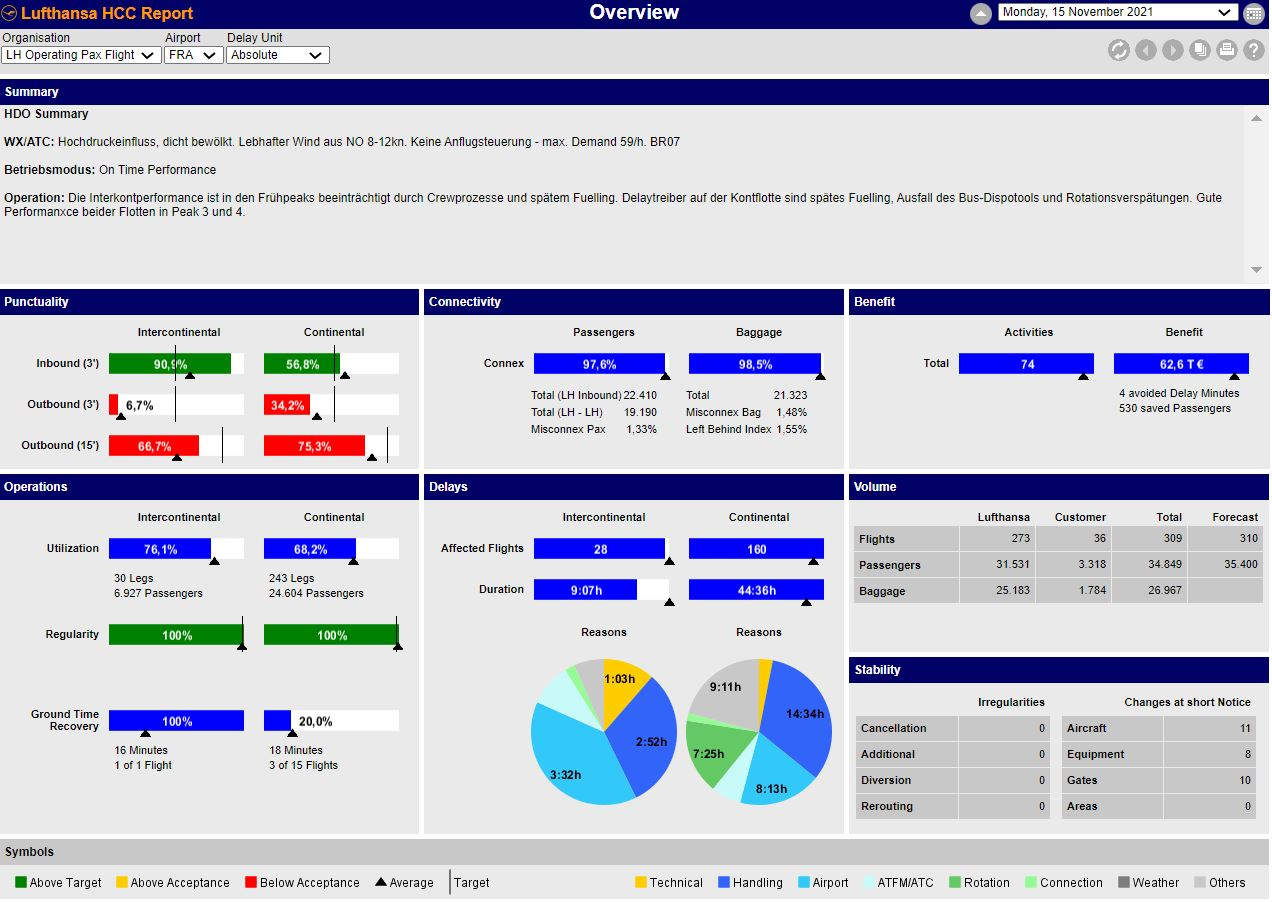
\includegraphics[width=1.5\textwidth]{./assets/obelisk-hcc.JPG}%
	}
\end{figure}
\newpage

\section{Obelisk Core - Explorer}
\label{appendix:obelisk_explorer}

\begin{figure}[htp]
	\makebox[\textwidth][c]{%
		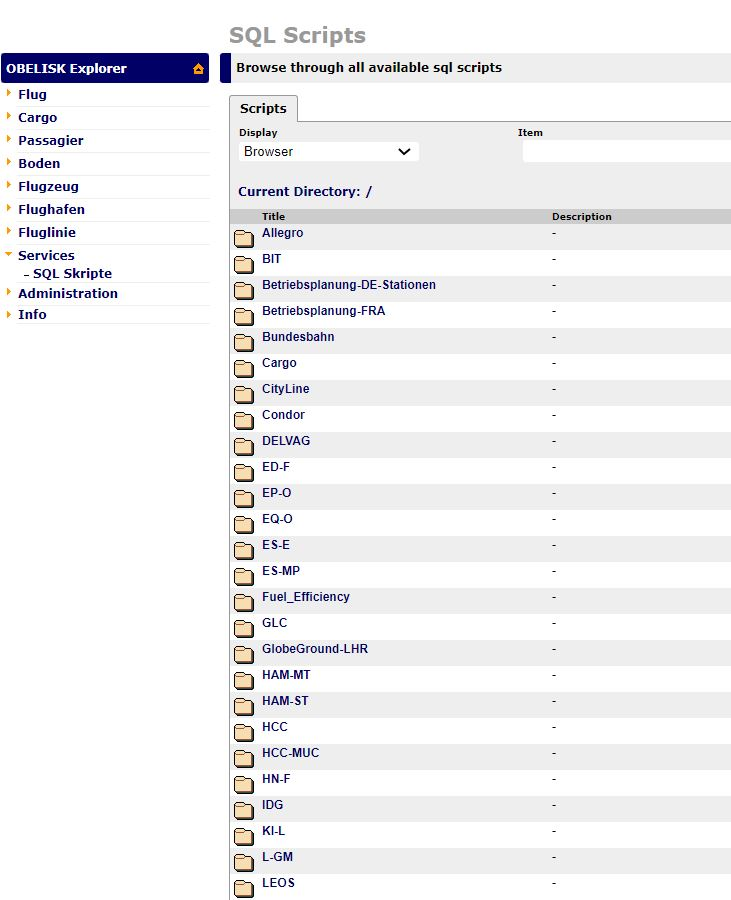
\includegraphics[width=1\textwidth]{./assets/obelisk-explorer.JPG}%
	}
\end{figure}
\newpage


\section{Obelisk Core - Selektionstool}
\label{appendix:obelisk_selektion}

\begin{figure}[htp]
	\makebox[\textwidth][c]{%
		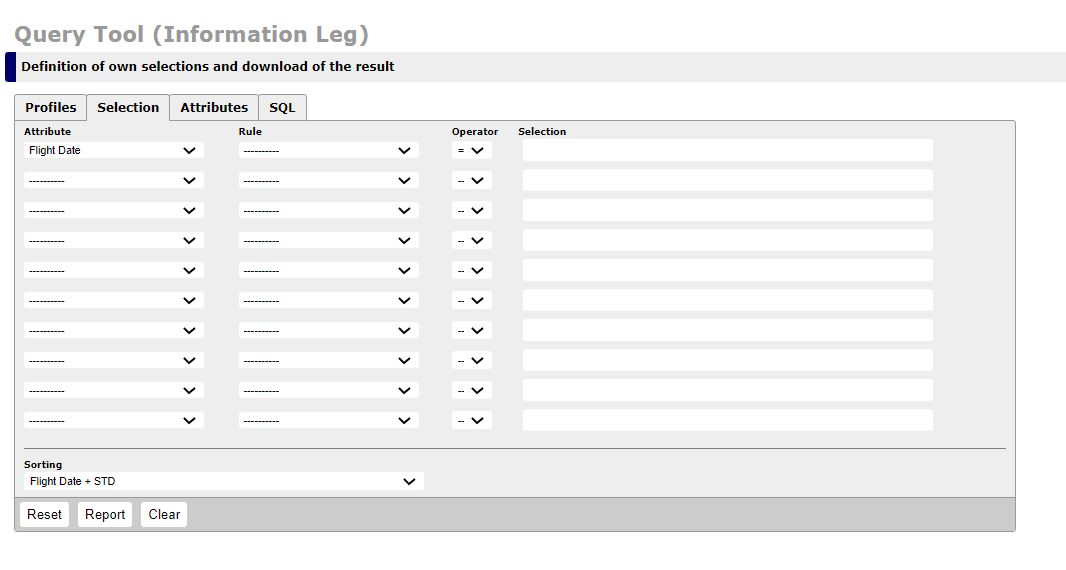
\includegraphics[width=1.5\textwidth]{./assets/obelisk-selektionstool.JPG}%
	}
\end{figure}
\newpage



\section{Tableau - DeepDives}
\label{appendix:tableau_deepdives}

\begin{figure}[h]
	\makebox[\textwidth][c]{%
		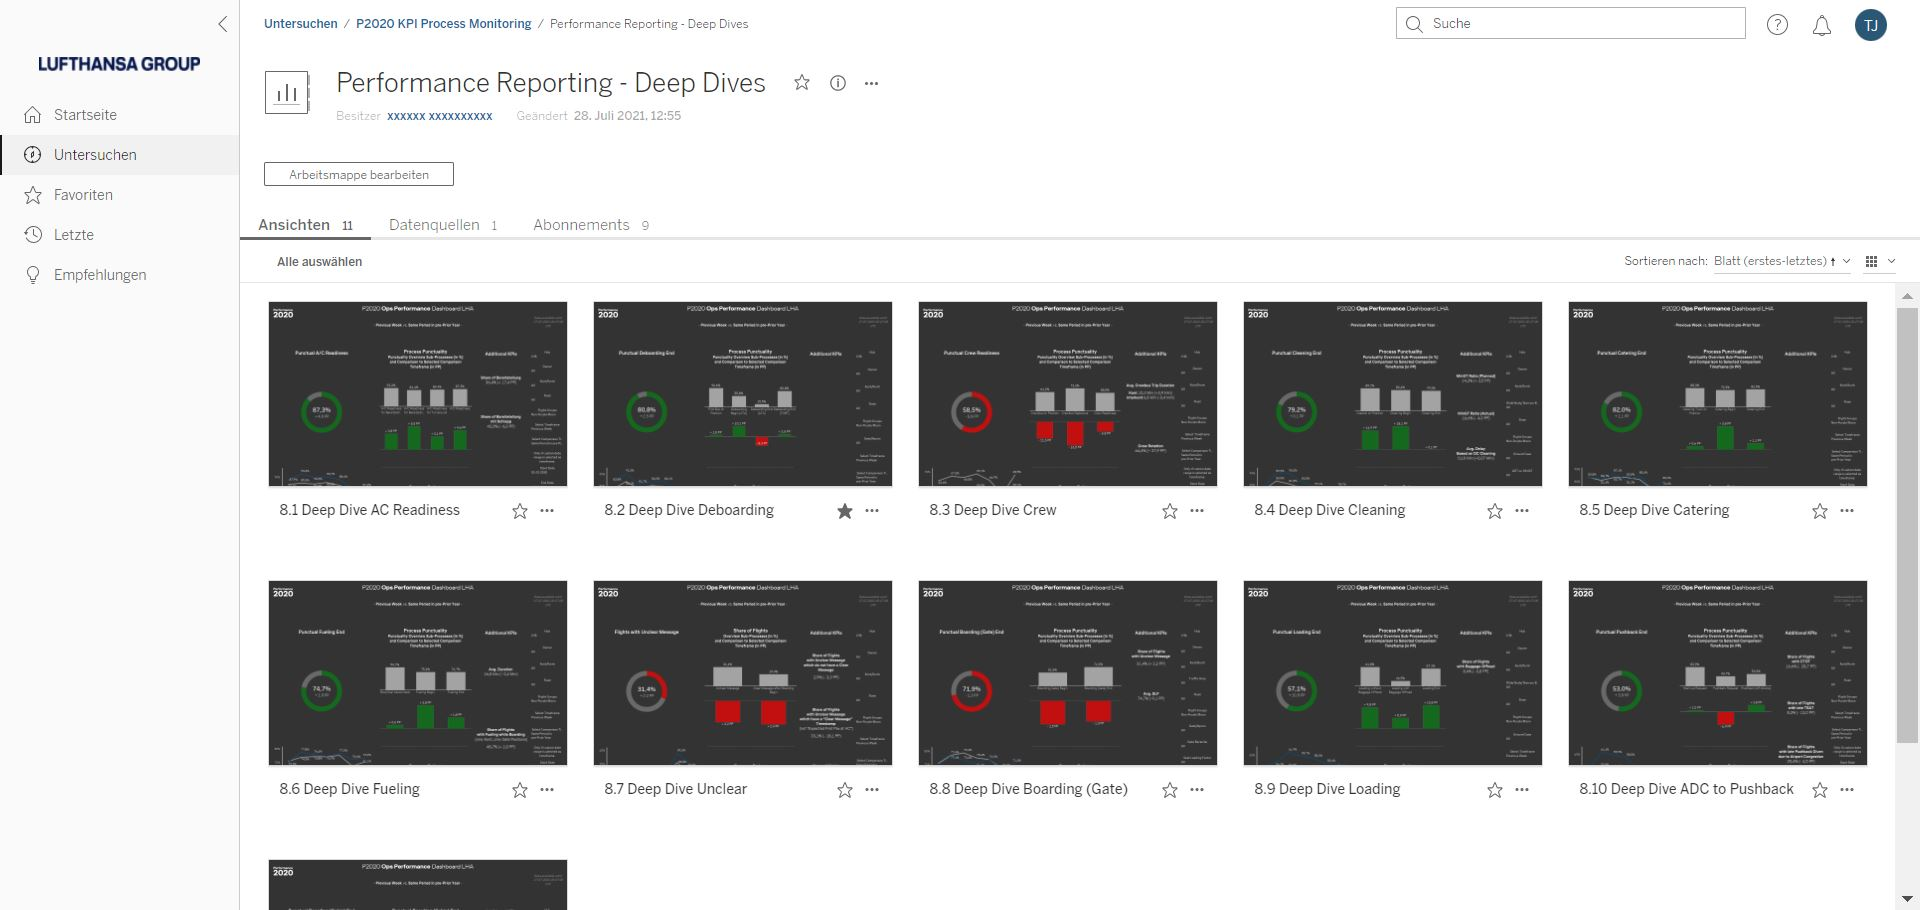
\includegraphics[width=1.5\textwidth]{./assets/tableau-deepdives.JPG}%
	}
\end{figure}
\newpage




\section{Tableau - DeepDive Deboarding}
\label{appendix:tableau_deepdive_deboarding}

\begin{figure}[h]
	\makebox[\textwidth][c]{%
		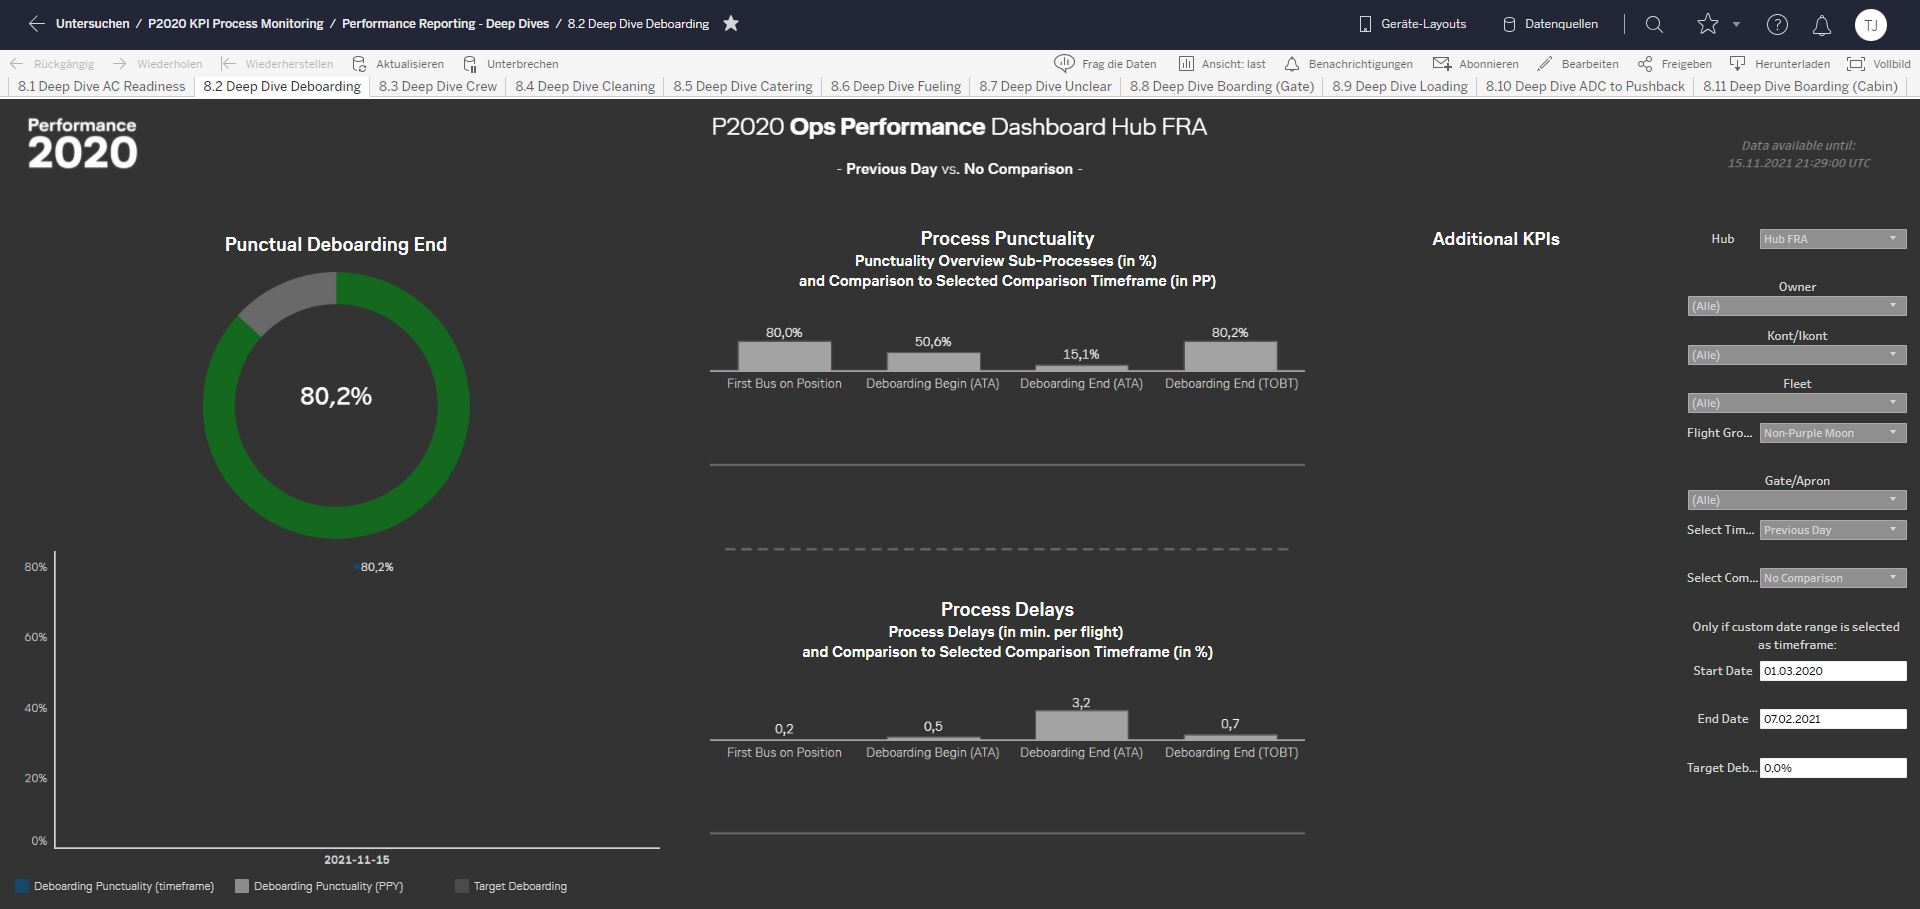
\includegraphics[width=1.5\textwidth]{./assets/tableau-deepdive-deboarding.JPG}%
	}
\end{figure}
\newpage


\section{Flight Operation Analyser - Filter}
\label{appendix:foa_filter}

\begin{figure}[h]
	\makebox[\textwidth][c]{%
		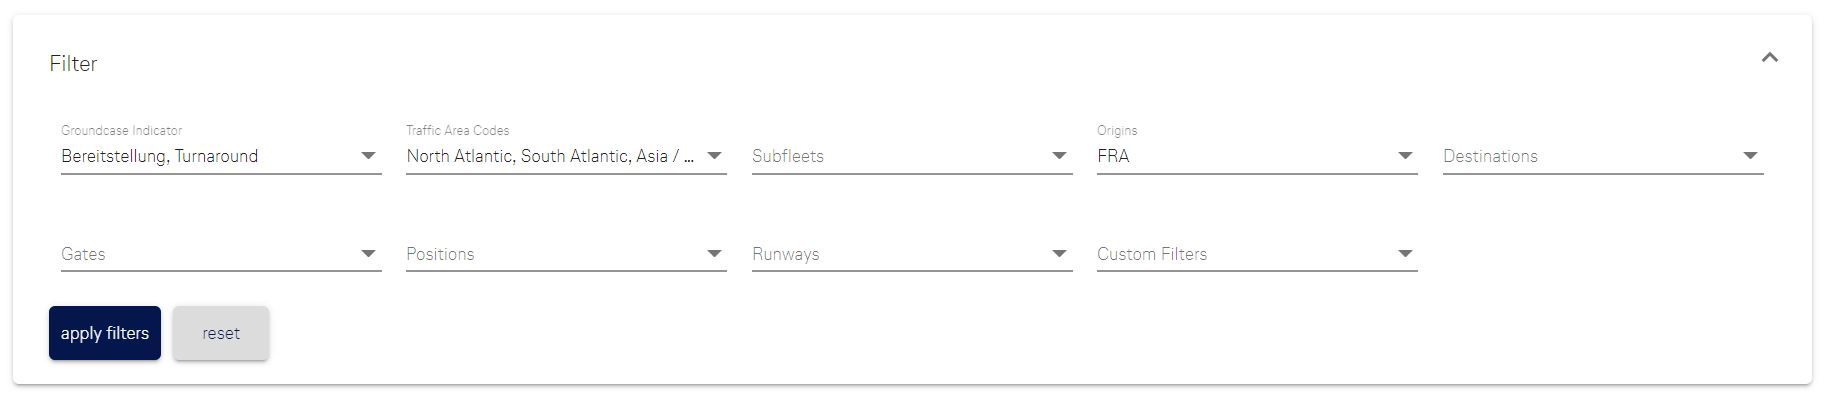
\includegraphics[width=1.5\textwidth]{./assets/foa-filter.JPG}%
	}
\end{figure}
\newpage



\section{Flight Operation Analyser - Filter - Selektion}
\label{appendix:foa_filter_2}

\begin{figure}[h]
	\makebox[\textwidth][c]{%
		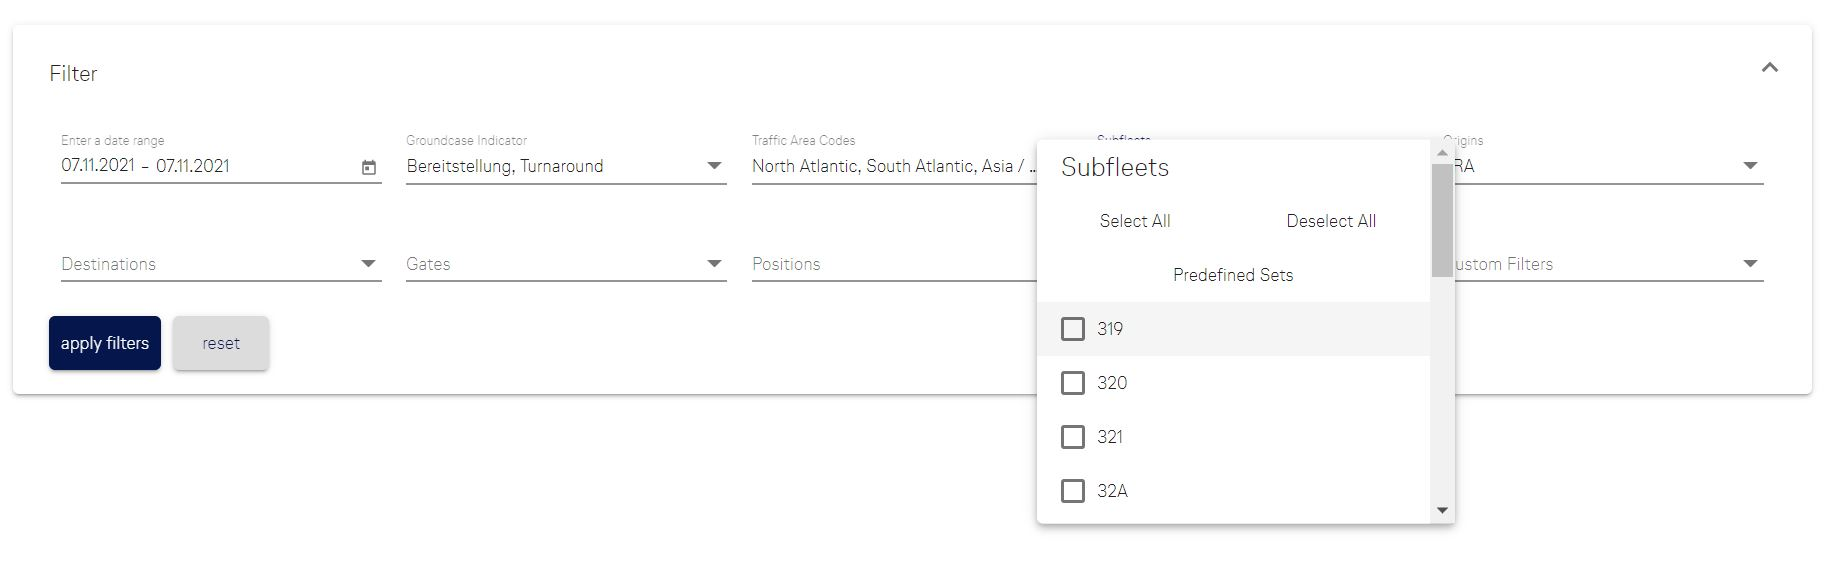
\includegraphics[width=1.5\textwidth]{./assets/foa-filter-2.JPG}%
	}
\end{figure}
\newpage


\section{Flight Operation Analyser - Filter - Vorgefertigte Sets}
\label{appendix:foa_filter_3}

\begin{figure}[h]
	\makebox[\textwidth][c]{%
		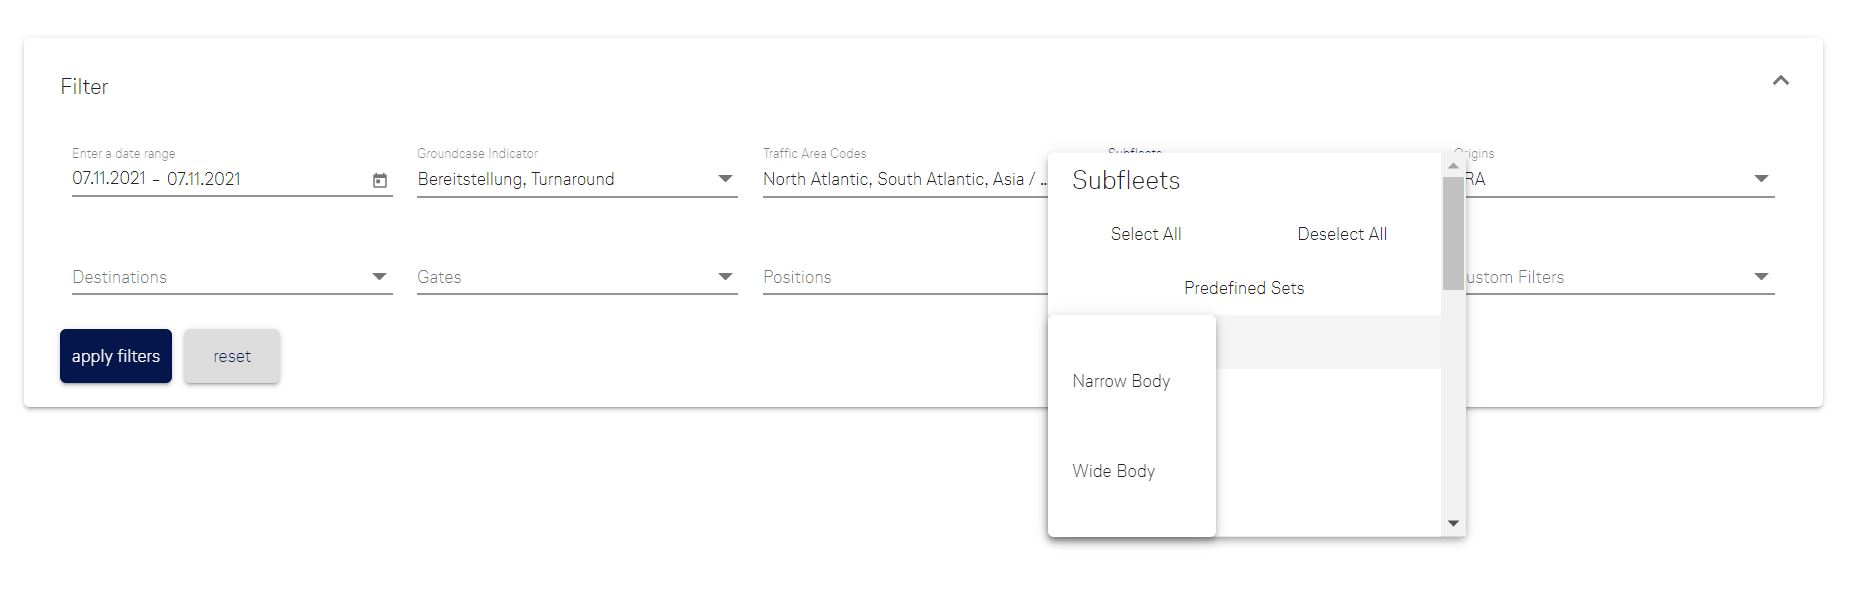
\includegraphics[width=1.5\textwidth]{./assets/foa-filter-3.JPG}%
	}
\end{figure}
\newpage


\section{Nutzwertanalyse}
\label{appendix:nutzwertanalyse}

\begin{figure}[h]
	\makebox[\textwidth][c]{%
		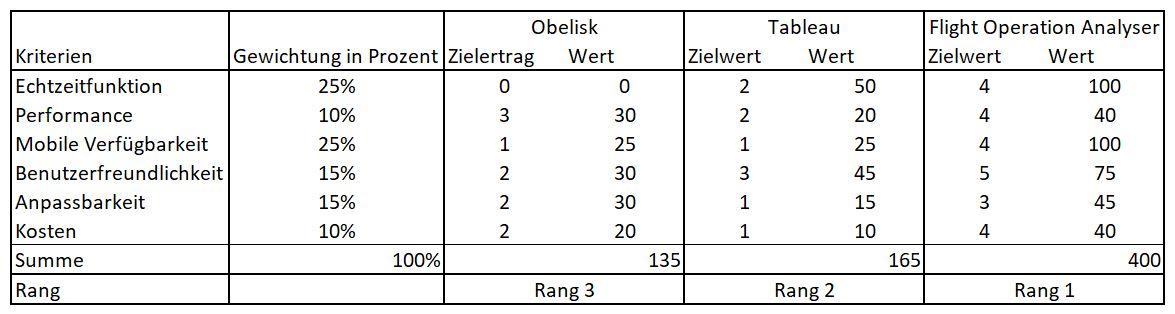
\includegraphics[width=1\textwidth]{./assets/nutzwertanalyse.JPG}%
	}
\end{figure}
\newpage

\section{MongoDB Model}
\label{appendix:mongoose_model}

\begin{figure}[h]
	\makebox[\textwidth][c]{%
		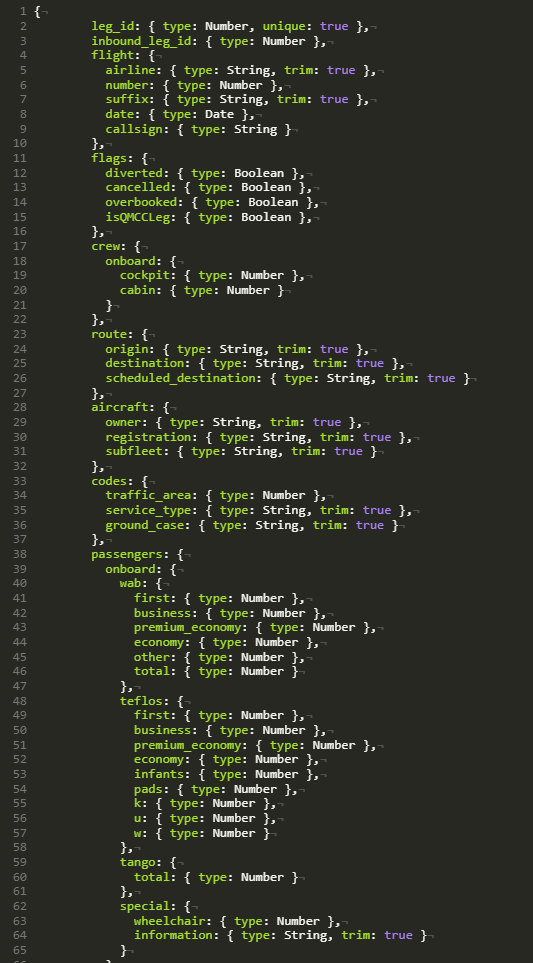
\includegraphics[width=0.65\textwidth]{./assets/model-1.png}%
	}
\end{figure}


\begin{figure}[h]
	\makebox[\textwidth][c]{%
	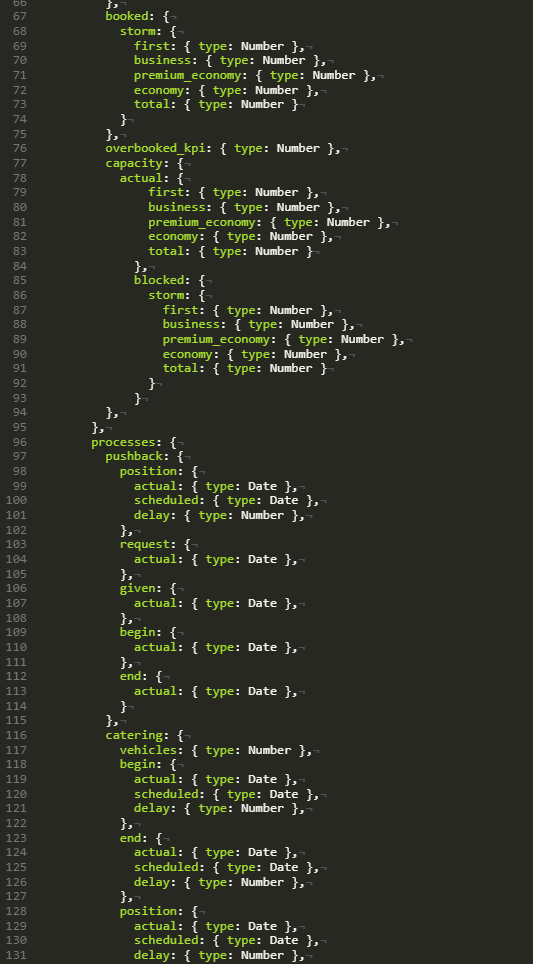
\includegraphics[width=0.65\textwidth]{./assets/model-2.png}%
	}
\end{figure}


\begin{figure}[h]
	\makebox[\textwidth][c]{%
	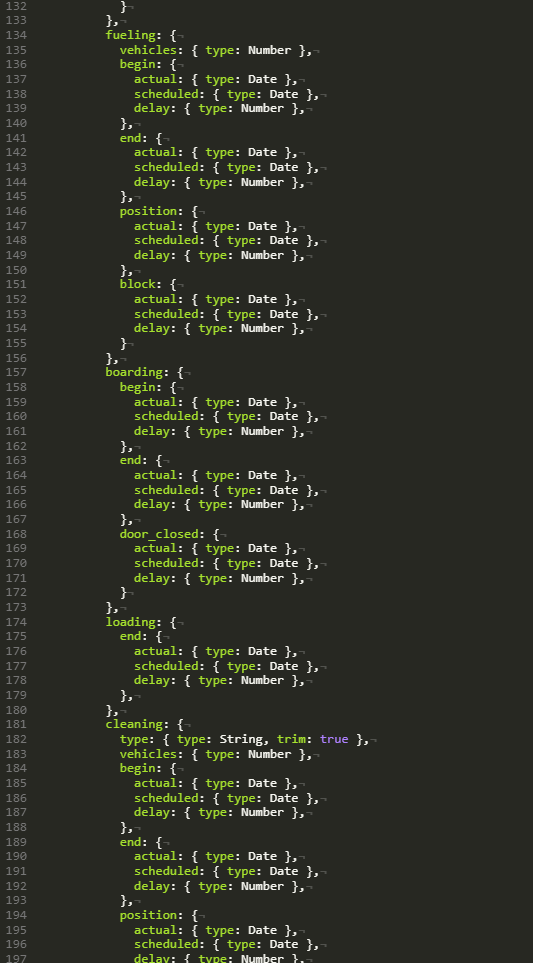
\includegraphics[width=0.65\textwidth]{./assets/model-3.png}%
	}
\end{figure}


\begin{figure}[h]
	\makebox[\textwidth][c]{%
	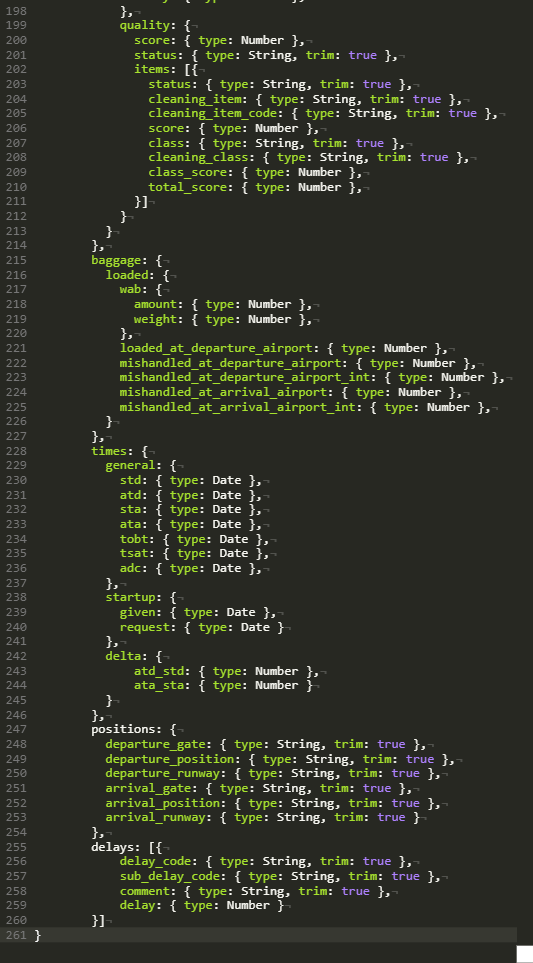
\includegraphics[width=0.65\textwidth]{./assets/model-4.png}%
	}
\end{figure}
\newpage

\end{appendices}